\documentclass[11pt,openany]{article}

\input{algebra-note-preamble}
\input{tcolorbox}
\input{theorem}
\input{algebra-note-commands}
\usepackage{tikz}
\usepackage{tikz-cd}
\usepackage{tikz-3dplot}
\usepackage{amsmath}
\usepackage{pgfplots}
\setstretch{1.25}
\begin{document}
\pagenumbering{arabic}
\begin{center}
	\huge\textbf{Category Theory, Presheaf and Sheaf}\\
	\vspace{0.5em}
	\large{Ji, Yong-hyeon}\\
	\vspace{0.5em}
	\normalsize{\today}\\
\end{center}
We cover the following topics in this note.
\begin{itemize}
	\item Category
	\item Functor
	\item Natural Transformation
	\item Determinant as Natural Transformation
	\item \st{Presheaf and Sheaf}
	\item TBA
\end{itemize}
\hrule\vspace{12pt}
\vfill
\section{Category, Functor and Natural Transformation}
\vfill
\begin{figure}[h!]\centering
	\adjustbox{scale=2}{
	\begin{tikzcd}
		A \arrow[rr, "f"] \arrow[rrdd, "g\circ f" description] \arrow["1_A"', loop, distance=2em, in=215, out=145] &  & B \arrow[dd, "g"] \arrow["1_B"', loop, distance=2em, in=35, out=325] \\
		&  &                                                                      \\
		&  & C \arrow["1_C"', loop, distance=2em, in=305, out=235]               
	\end{tikzcd}}
\caption{Category}
\end{figure}

\newpage
\defbox[Category]{\begin{definition}
A \textbf{category} $\mathcal{C}$ consists of the following data: \begin{enumerate}[(i)]
\item (\textbf{Objects}) A class $\boxed{\text{Ob}(\mathcal{C})}$, whose elements are called \textbf{objects} of category $\mathcal{C}$.
\item (\textbf{Morphisms}) For each pair of objects $A,B\in\text{Ob}(\mathcal{C})$ , a class $\boxed{\text{Mor}_\mathcal{C}(A,B)}$\footnote{Sometimes, we also denote it by $\text{Hom}(A,B)$ or $\mathcal{C}(A,B)$.}, whose elements are called \textbf{morphisms} (or \textbf{arrows}) from $A$ to $B$.
\item (\textbf{Composition}) For any $f\in\text{Mor}_\mathcal{C}(A,B)$ and $g\in\text{Mor}_\mathcal{C}(B,C)$, a \textbf{composition} $$\boxed{(g\circ f)\in\text{Mor}_\mathcal{C}(A,C)}.$$
\end{enumerate}
These data are to satisfy the following axioms:
\begin{enumerate}[1.]
\item (\textbf{Identity}) For every object $A\in\text{Ob}(\mathcal{C})$, there exists an \textbf{identity morphisms} $$\boxed{1_A\in\text{Mor}_\mathcal{C}(A,A)}.$$
%such that for any $f\in\text{Mor}_{\mathcal{C}}(A,B)$ and $g$.
\item (\textbf{Associativity}) For any $f\in\text{Mor}_{\mathcal{C}}(A,B),g\in\text{Mor}_{\mathcal{C}}(B,C)$,
and $h\in\text{Mor}_{\mathcal{C}}(C,D)$, \[
\boxed{h\circ(g\circ f)=(h\circ g)\circ f}.
\]
\end{enumerate}
\end{definition}}
\begin{remark}
	\ \\\begin{figure}[h!]
		\centering
		\begin{minipage}{.48\textwidth}\centering% https://tikzcd.yichuanshen.de/#N4Igdg9gJgpgziAXAbVABwnAlgFyxMJZABgBpiBdUkANwEMAbAVxiRAEEQBfU9TXfIRQAmclVqMWbAELdeIDNjwEio4ePrNWiEAGFu4mFADm8IqABmAJwgBbJGRA4ISAIzUGWMNpBQ6cAAsjEGpNKR0LOUsbe0R3JxdEURBPbzY-QODQyR9jKJBrOwdqZyRksNyAHUqAYywrGoACSI86ACMYBgAFfmUhECssYwCcAy4gA
			\adjustbox{scale=.9}{\begin{tikzcd}
				A \arrow[rr, "f", dashed] \arrow[rrdd, "g\circ f"'] &  & B \arrow[dd, "g", dashed] \\
				&  &                           \\
				&  & C                        
			\end{tikzcd}}\caption{Composition of Morphisms}
		\end{minipage}%
		\begin{minipage}{.48\textwidth}\centering% https://tikzcd.yichuanshen.de/#N4Igdg9gJgpgziAXAbVABwnAlgFyxMJZABgBpiBdUkANwEMAbAVxiRAEEQBfU9TXfIRQAWclVqMWbAELdxMKAHN4RUADMAThAC2SMiBwQkARmoMsYVohBwI5qCGr1mVkGoC8agDpeAxlg1fAAIfHBgADxw4NWAsKC4AfU5qOAALLDUcJABaACYedS1dRFMDI0R9NIysxDynSVdFd1CIqJi4xPYff0CgxW5eNyK9akMRkAYICDQiYwAOMjVGOBhxBjoAIxgGAAV+PAI2DSxFVKz6lzYWyOjY+KSBwp0TUfLSyemiReXVs03tvbYA5CEDHU7nCSXazXNp3RKyLgULhAA
			\adjustbox{scale=.9}{\begin{tikzcd}
				A \arrow[rrrr, "f=f\circ 1_A", shift left=2] \arrow["1_A"', loop, distance=2em, in=125, out=55] &  &  &  & B \arrow[llll, "g=1_A\circ g", shift left=2] \arrow["1_B"', loop, distance=2em, in=305, out=235]
			\end{tikzcd}}\caption{Identity Morphisms}
		\end{minipage}%
	\end{figure}
	\begin{figure}[h!]\centering% https://tikzcd.yichuanshen.de/#N4Igdg9gJgpgziAXAbVABwnAlgFyxMJZABgBpiBdUkANwEMAbAVxiRAEEQBfU9TXfIRQAmclVqMWbAMLdeIDNjwEiARjHV6zVohAAhOXyWCiAZg0TtbACLdxMKAHN4RUADMAThAC2SMiBwIJFFLKV03QxBPH2DqQKR1UJ0QR0jo30RE+MRzJLYACzSvDP9sxIAjGDAoJAAWAE5NSWTHAB1WgGMsDw6AAgied2K-OKCc6krqpAA2fy0wkHz2rp6ACjbO7r63AEoimMQQ7NzJmsQAWgamq10lzZ7e1OoGOkqGAAV+ZSEQDyxHfI4fYlUZIE5VM7nWbXBarO4rPqOHbLLb9EDUOD5LBuIGIfwvN6fYwqXR-AFArgULhAA
		\adjustbox{scale=.9}{\begin{tikzcd}
			A \arrow[r, "f"] \arrow[rr, "g\circ f", bend left=49] \arrow[rrr, "h\circ(g\circ f)", bend left=60] \arrow[rrr, "(h\circ g)\circ f"', bend right=60] & B \arrow[r, "g"] \arrow[rr, "h\circ g"', bend right=49] & C \arrow[r, "h"] & D
		\end{tikzcd}}\caption{Associativity of Composition}
	\end{figure}
\end{remark}

\newpage
\begin{example}
\ \begin{table}[h!]\centering\setstretch{1.5}
\begin{tabular*}{\textwidth}{@{\extracolsep{\fill}}lcr}\hline
	\textbf{Category} & \textbf{Object} & \textbf{Morphism} \\ \hline\hline
	$\mathscr{S}$et & Sets & Functions between sets \\ \hline
	$\mathscr{G}$roup & Groups & Group Homomorphisms \\ \hline
	$\mathscr{R}$ing & Rings & Ring Homomorphisms \\ \hline
	$\mathscr{V}$ector Space & Vector Spaces & Linear Transformations \\ \hline
	$\mathscr{T}$opology Space & Topological Spaces & Continuous Maps \\ \hline
	$\mathscr{P}$oset & Partially Ordered Sets & Order-preserving Maps \\ \hline
	$\vdots$ & $\vdots$ & $\vdots$ \\ \hline
\end{tabular*}
\end{table}
\end{example}
\vfill
\defbox[Functor]{\begin{definition}
A \textbf{functor} $\mathbf{F}:\mathcal{C}\to\mathcal{D}$ is a mapping between two categories $\mathcal{C}$ and $\mathcal{D}$ is given by the following data: \begin{enumerate}[(i)]
	\item (\textbf{Object Mapping}) A mapping that assign to each object $A\in\text{Ob}(\mathcal{C})$ an object $\textbf{F}(A)\in\text{Ob}(\mathcal{D})$: \[
	\fullfunction{\textbf{F}}{\text{Ob}(\mathcal{C})}{\text{Ob}(\mathcal{D})}{A}{\textbf{F}(A)}
	\]
	\item (\textbf{Morphism Mapping}) For each pair $A,B\in\text{Ob}(\mathcal{C})$, a mapping that assigns to each morphism $\phi\in\text{Mor}_{\mathcal{C}}(A,B)$ a morphism $\textbf{F}(\phi)\in\text{Mor}_{\mathcal{D}}(\textbf{F}(A),\textbf{F}(B))$: \[
	\fullfunction{\textbf{F}}{\text{Mor}_{\mathcal{C}}(A,B)}{\text{Mor}_{\mathcal{D}}(\textbf{F}(A), \textbf{F}(B))}{\phi}{\textbf{F}(\phi)}
	\]
\end{enumerate}
\end{definition}}
\begin{remark}[Compatibility with Identity Morphisms and Composition]
	These functors satisfy the following conditions:
	\begin{enumerate}[1.]
		\item (\textbf{Preservation of Identity Morphisms}) For every object $A\in\text{Ob}(\mathcal{C})$, \[
		\textbf{F}(1_A)=1_{\textbf{F}(A)}.
		\]
		\item (\textbf{Preservation of Composition}) For all morphisms
		$\phi\in\text{Mor}_{\mathcal{C}}(A,B)$ and $\psi\in\text{Mor}_{\mathcal{C}}(B,C)$, \[
		\textbf{F}(\psi\circ\phi) = \textbf{F}(\psi)\circ \textbf{F}(\phi).
		\]
	\end{enumerate}
\end{remark}
\newpage
\begin{remark}
\	\begin{center}% https://tikzcd.yichuanshen.de/#N4Igdg9gJgpgziAXAbVABwnAlgFyxMJZABgBpiBdUkANwEMAbAVxiRAEEQBfU9TXfIRQAmclVqMWbAELdeIDNjwEio4ePrNWiEAGE5fJYKIA2MdU1SdAHWs4YADxwAjAGbAAYlwAU7AJQGCvzKQsgAHOYSWmy29k5unj7SATyGAiooEeoWktogsY4u7l7euinyiumhAMykAIwauWyBlSFEAKz1jdE63OIwUADm8ESgrgBOEAC2SGQgOBBIdTk9+dZoABZYgRPTS9QLSKJRVmto2DuTM4hzh4jHlnm251i2AMZY42-PWyDUDHRnDAGAAFYLGHTjLCDDY4S57G4HRaIkAMCAQNCqADsZFcjDgMHEAKBoPBGRAUJhcJWpzqAH1OKkQLtrst5si2WiMUQAJy4-GE-6A4Fgozkymwv4nPL02RMllHJGK1HozEofkMAlE4WksVCCnQyU0mV0-Tyq5IWrspAAFmNMTshQSJR+WHKYwtiDt1sQnWlDriRUS3me2HdzM9VrufseAadxR8ode1g+X1dfgAvAV4gmQ+sw+9Pt9HTng+mpcSRWT9RK4eaEVHkVauWrkMIcaQ8ZrBaidaKqmxa1LYzp6cBs0GSv4uPDrt67t6W7yNVqhST+21IYbqf7R3TxyXJ0k-DP69c-dH-qqiCue5XdQOt1Th009wfA86fGUZ-8sGA8nAEAMFgUBShsMB0KBiBgEwDAMAcdBYAwbCQP+s5IGYPpYvaNiHp+FZ-gBQEgX0XBAA
	\begin{tikzcd}[remember picture]
		A \arrow[rr, "\phi"] \arrow[rrdd, "\psi\circ\phi"'] \arrow["1_A"', loop, distance=2em, in=215, out=145] &  & B \arrow[dd, "\psi"] \arrow["1_B"', loop, distance=2em, in=35, out=325] &                             &  &    & \textbf{F}(A) \arrow[rr, "\textbf{F}(\phi)"] \arrow[rrdd, "\textbf{F}(\psi\circ\phi)=\textbf{F}(\psi)\circ\textbf{F}(\phi)"'] \arrow["1_{\textbf{F}(A)}"', loop, distance=2em, in=215, out=145] &  & \textbf{F}(B) \arrow[dd, "\textbf{F}(\psi)"] \arrow["1_{\textbf{F}(B)}"', loop, distance=2em, in=35, out=325] \\
		&  &                                                                         & {} \arrow[rr, "\textbf{F}"] &  & {} &                                                                                                                                                                                                 &  &                                                                                                               \\
		&  & C \arrow["1_C"', loop, distance=2em, in=305, out=235]                   &                             &  &    &                                                                                                                                                                                                 &  & \textbf{F}(C) \arrow["1_{\textbf{F}(C)}"', loop, distance=2em, in=305, out=235]                              
	\end{tikzcd}
	
\begin{tikzpicture}[overlay,remember picture]
%	\def \xMax{0}
%	\def \xMin{-14}
%	\def \yMax{4}
%	\def \yMin{-4}
%	\draw[very thin,color=gray!15,step=.5] (\xMin,\yMin) grid (\xMax,\yMax);
%	
%	\foreach \i in {\xMin,...,-2,-1,1,2,...,\xMax}
%	\draw[gray] (\i,.1)--(\i,-.1) node[below] {$\i$};%x-axis
%	\foreach \i in {\yMin,-1,1,1,\yMax}
%	\draw[gray] (.1,\i)--(-.1,\i) node[left] {$\i$};%y-axis
	
	\draw[dotted, red, line width=.5mm] (-14,-2.5) rectangle (-8.75,2) node[above] {Category $\mathcal{C}$};
	\draw[dotted, red, line width=.5mm] (-6.5,-2.5) rectangle (0,2) node[above] {Category $\mathcal{D}$};
	\end{tikzpicture}
	\end{center}
\ \begin{center}
% https://tikzcd.yichuanshen.de/#N4Igdg9gJgpgziAXAbVABwnAlgFyxMJZABgBpiBdUkANwEMAbAVxiRAEEQBfU9TXfIRRkATFVqMWbAELdeIDNjwEiAFnLj6zVohAAdPThgAPHACMAZsABiXABTsAlHL5LBa0mOpapug0dNLG3tpZx5XARVhUgBGTUkdEBcFfmUhZHU47wS2bnEYKABzeCJQCwAnCABbJDIQHAgkGOztNgM0AAssEGoGOjMYBgAFVPddcqxCjpxkiuqkEWoGpABmFt99QxNzK1s7dq7nXv7BkbcokAmpmfCQOZrEOuXERZAGLDBEqAgcIygekADMD-RArOp9AbDUYXBgwCwzdaJfzbIK2WaVB7NeqNUGItpbQK7LgAoEggC0YN6Hy+Pz+6PmiHU2KQAFYqZ82N9fgUAT4kQSdsESTBgas6nAuvCkBSuBQuEA
\begin{tikzcd}
	A \arrow[dd, "\phi"'] \arrow[rrrr, "\textbf{F}", dotted, bend left] &  &  &  & \textbf{F}(A) \arrow[dd, "\textbf{F}(\phi)"'] \\
	{} \arrow[rrrr, "\textbf{F}", dotted, bend left, shift left=3]      &  &  &  & {}                                            \\
	B \arrow[rrrr, "\textbf{F}", dotted, bend right]                    &  &  &  & \textbf{F}(B)                                
\end{tikzcd}
\end{center}
\end{remark}

\begin{example}
\ \begin{table}[h!]\centering\setstretch{1.5}
	\adjustbox{width=\textwidth}{\begin{tabular}{lcccr}\hline
		\textbf{Category (Source)} & \textbf{Functor} & \textbf{Object Mapping} & \textbf{Morphism Mapping} & \textbf{Category (Target)} \\ \hline\hline
%		$\mathscr{S}$et & Identity Fuctor $\textbf{Id}_{\mathscr{S}et}$ & $X\mapsto X$ & $(f:X\to Y)\mapsto (f:X\to Y)$ & $\mathscr{S}$et \\ \hline
		TBA & TBA & TBA & TBA & TBA \\
%		$\mathscr{S}$et & Identity Fuctor $\textbf{Id}_{\mathscr{S}et}$ & $X\mapsto X$ & $(f:X\to Y)\mapsto (f:X\to Y)$ & $\mathscr{S}$et \\ \hline
%		\multirow{2}{*}{$\mathscr{S}$et} & Power Set Functor & $X\mapsto P(X),$ & $(f:X\to Y)\mapsto (P(f):P(X)\to P(Y))$, & $\mathscr{S}$et \\ 
%		& $P:\mathscr{S}$et$\to$$\mathscr{S}$et & where $P(X)=\set{A:A\subseteq X}$ & where $P(f)(A)=\set{f(a):a\in A}$ &\\ \hline
%		$\mathscr{G}$roup & Groups & Group Homomorphisms \\ \hline
%		$\mathscr{R}$ing & Rings & Ring Homomorphisms \\ \hline
%		$\mathscr{V}$ector Space & Vector Spaces & Linear Transformations \\ \hline
%		$\mathscr{T}$opology Space & Topological Spaces & Continuous Maps \\ \hline
%		$\mathscr{P}$oset & Partially Ordered Sets & Order-preserving Maps \\ \hline
		$\vdots$ & $\vdots$ & $\vdots$ & $\vdots$ & $\vdots$ \\ \hline
	\end{tabular}}
\end{table}
\end{example}

\newpage
\defbox[Natural Transformation]{\begin{definition}
Let $\mathcal{C}$ and $\mathcal{D}$ be categories, and let $\textbf{F},\textbf{G}:\mathcal{C}\to\mathcal{D}$ be two functors. A \textbf{natural transformation} (or a \textbf{morphism of functors}) $\eta:\textbf{F}\Rightarrow\textbf{G}$, is a collection $\set{\eta_A}_{A\in\text{Ob}(\mathcal{C})}$ such that \begin{enumerate}[(i)]
	\item (\textbf{Component Morphisms}) For each object $A\in\text{Ob}(\mathcal{C})$, there is a morphism \[
	\eta_A:\textbf{F}(A)\to\textbf{G}(A)
	\] in the category $\mathcal{D}$, called the \textbf{component of $\eta$ at $A$}.
	\item (\textbf{Naturality Condition}) For each morphism $\phi:A\to B$ in $\mathcal{C}$ the following diagram in $\mathcal{D}$ commutes:
	\begin{center}
		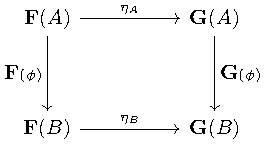
\includegraphics[scale=1.25]{./nt.pdf}
	\end{center}
\end{enumerate}
In other words, \[
\eta_B\circ\textbf{F}(\phi)=\textbf{G}(\phi)\circ\eta_A
\] for all $\phi:A\to B$ in $\mathcal{C}$.
\end{definition}}
\begin{remark}
Sometimes we use the diagram
\begin{center}
	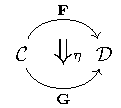
\includegraphics[scale=1.25]{./nt2.pdf}
\end{center}
to indicate that $\eta$ is a morphism form $\textbf{F}$ to $\textbf{G}$.
\end{remark}
\vspace{24pt}
%\begin{remark}
%	A natural transformation $\eta:\textbf{F}\Rightarrow\textbf{G}$ is a ``morphism of functors'' that provides a way to compate the actions of $\textbf{F}$ and $\textbf{G}$ on both objects and morphisms of $\mathcal{C}$, ensuring compatibility with the categorical structure of $\mathcal{C}$ and $\mathcal{D}$.
%\end{remark}
\newpage
\begin{remark}
\ \\ \adjustbox{scale=1.25, center}{
% https://tikzcd.yichuanshen.de/#N4Igdg9gJgpgziAXAbVABwnAlgFyxMJZABgBpiBdUkANwEMAbAVxiRAEEQBfU9TXfIRRkATFVqMWbAELdeIDNjwEiI8uPrNWiEAB1dAWzo4AFgCMAZsABiXABTsAlHL5LBq0mOqapO-UdNLG3tpZx5XARUUABZ1b0ltPUNjcysAcXsnFwV+ZSFkWK8JLTZ-FKCMu1DsxUj8sgBGDQS2Gtz3FDUm+JKdNrcogtJu4t8QbnEYKABzeCJQCwAnCAMkMhAcCCQGnrH9NBMsEGoGOjMYBgAFdqiQRaxpkxxspZWkNQ2txABmXcT97AAXjKgSstjs+0OzhOZwu1wGQhADBgFme4RAr1WiFinyQAFY-qVdABjQ7A5Kg4CVSFYaFI2FXG6I5Gol7LLEfTZIHE+f66GA4OgAfU46MxSF+uMQBNGfIFwtkYvZa2oXOx1HOYCg3IAnCcsGBElAIDgcFNjrKiQFUlSuBa4IdWYgALQfU7nRkItgG7CwNlvRDrNUfXlW8pgu36w1sY2m80amBaiXrd1wpnesC+1hKgM7KWShgGo0ms3ahNJl3fdahvwUm22C2pz11DNZ-1YvNqmWa7Uu6J6kAOrBOlNFmMl+P0j3wls6H1YP2E2vWip2nNYgBsqq+AHYo8W42XLcvw8F7Y7nn2YdP03PMwvs-JxYgt1KABz78eHi01pIr9KRoOF7cteaZenebZcBQXBAA
\begin{tikzcd}
	A \arrow[dd, "\phi"'] \arrow[rrrr, "\mathbf{G}" description, dotted, bend left=49, shift left=2] \arrow[rr, "\mathbf{F}" description, dotted, bend left] &  & \mathbf{F}(A) \arrow[dd, "\psi=\mathbf{F}(\phi)"] \arrow[rr, "\eta_A"] &  & \mathbf{G}(A) \arrow[dd, "\chi=\mathbf{G}(\phi)"] \\
	{} \arrow[rr, "\mathbf{F}" description, dotted, shift left=4] \arrow[rrrr, "\mathbf{G}" description, dotted, shift right=4]                              &  & {}                                                                     &  & {}                                                \\
	B \arrow[rr, "\mathbf{F}" description, dotted, bend right] \arrow[rrrr, "\mathbf{G}" description, dotted, bend right=49]                                 &  & \mathbf{F}(B) \arrow[rr, "\eta_B"]                                     &  & \mathbf{G}(B)                                    
\end{tikzcd}}
\end{remark}
\vfill
\begin{example}[Determinant]
We start with the basic concepts and gradually introduce the determinant as a mathematical object.
\begin{enumerate}[\bf \text{Step} 1.]
	\item \textbf{\large Understanding Matrices.} 
	
	A matrix is a rectangular array of numbers. For example, a $2\times 2$ matrix look like this:\[
	A=\begin{pmatrix}
		a & b \\ c & d
	\end{pmatrix},
	\] where $a,b,c,d$ are numbers.
%	Matrices can represent transformations of space, such as stretching, rotating, or squashing.
	\item \textbf{\large Invertibility of Matrices.} The inverse of 
	$A=\begin{pmatrix}a & b \\ c & d\end{pmatrix}\in M_2(\R)$ (if it exists) is given by: \[
	A^{-1}=\frac{1}{\textcolor{blue}{ad-bc}}\begin{pmatrix}
		d & -b \\ -c & a
	\end{pmatrix}.
	\] The \textcolor{blue}{determinant} is a single number associated with a matrix, defined for $2\times 2$ matrices as: \[
	\det\begin{pmatrix}
		a & b \\ c & d
	\end{pmatrix}=ad-bc.
	\]
	\item \textbf{\large The Determinant as a Function from $M_2(\mathbb{R})$ to $\mathbb{R}$}
	
	The set $M_2(\R)$ is the set of all $2\times 2$ matrices with real entries: \[
	M_2(\R):=\set{\begin{pmatrix}
		a & b \\ c & d
	\end{pmatrix}:a,b,c,d\in\R}.
	\] The determinant is a function: \[
	\fullfunction{\det}{M_2(\R)}{\R}{A}{\det(A)=ad-bc\in\R}
	\] for each $A=\begin{pmatrix}
		a & b \\ c & d
	\end{pmatrix}\in M_2(\R)$. This function assigns a real number to each $2\times 2$ matrix.
	\item \textbf{\large Properties of the Determinant Function.}
	\begin{itemize}
%		\item (\textbf{Additivity}) The determinant is linear in each row when the other row is fixed.
		\item (\textbf{\color{red} Multiplicativity}) For any $A,B\in M_2(\R)$, \[
		\det(A*B)=\det(A)\cdot\det(B)
		\] with $*$ is matrix multiplication and $\cdot$ is number multiplication.
		\item (\textbf{Normalization}) The determinant of the identity matrix is: \[
		\det\begin{pmatrix}
			1 & 0 \\ 0 & 1
		\end{pmatrix}=1.
		\]
	\end{itemize}
	\item \textbf{\large Group Structure}
	
	We identify a natural subset of $M_2(\R)$ where: \begin{itemize}
		\item The determinant is nonzero.
		\item  The operation of matrix multiplication is preserved.
	\end{itemize}
	\begin{enumerate}[1.]
		\item (Closure Under Multiplication) For $A,B$ in this subset, their product is also a $2\times 2$ matrix. Using the determinant property, \[
		\det(A)\neq 0\land \det(B)\neq 0\implies \det(AB)=\det(A)\det(B)\neq 0.
		\]
		\item (Associativity) Matrix multiplication is associative.
		\item (Existence of Identity and Inverses) The identity matrix $I=\begin{pmatrix}
			1 & 0 \\ 0 & 1
		\end{pmatrix}$ satisfies $\det(I)=1\neq 0$, and for every matrix $A$ in this subset, there exists $A^{-1}$ since $\det(A)\neq 0$.
	\end{enumerate}
	These properties define a group, and this subset of matrices is precisely the general linear group of invertible matrices: \[
	\text{GL}(2,\R):=\set{A\in M_2(\R),\det(A)=ad-bc\neq 0}.
	\]
	\vfill
	\item \textbf{\large The Determinant as a Group Homomorphism from $\text{GL}(2,\R)$ to $\R^\times$}
	
	The determinant is restricted to invertible matrices:
	\[
	\det:\text{GL}(2,\R)\to \R^{\times},
	\] where $\R^{\times}$ is the set of nonzero real numbers under multiplication. The determinant preserves the group operation because because of the multiplicative property: \[
	\det(A*B)=\det(A)\cdot\det(B).
	\] for all $A,B\in\text{GL}(2,\R)$. 
	\vfill
	\item \textbf{\large Matrices Over a Commutative Ring}
	
	Let $R$ be a commutative ring. The determinant of $A\in M_2(R)$ is define as \[
	\det A = a\cdot d + (-(b\cdot c)),
	\] using the addition and multiplication operations of the commutative ring $R$.
	\vfill
	\item \textbf{\large Categories}
	\begin{itemize}
		\item The Category $\mathsf{CRing}$: The Category of Commutative Rings
		\begin{itemize}
			\item Objects: commutative rings
			\item Morphisms: ring homomorphisms
			\item Composition: standard composition of functions
			\item Identity Morphisms: $1_R:R\to R$ defined by $1_R(a)=a$ for $a\in R$
		\end{itemize}
		\item The Category $\mathsf{Grp}$: The Category of Groups
		\begin{itemize}
			\item Objects: groups
			\item Morphisms: group homomorphisms
			\item Composition: standard composition of functions
			\item Identity Morphisms: $1_G:G\to G$ defined by $1_G(a)=a$ for $a\in G$
		\end{itemize}
	\end{itemize}
	\newpage
	\item \textbf{\large Functors}
	\begin{itemize}
		\item The General Linear Group Functor $\mathbf{GL}_2$
		\begin{itemize}
			\item $R\mapsto \textbf{GL}_2(R)$
			\item $(\phi:R\to S)\mapsto (\textbf{GL}_2(\phi):\textbf{GL}_2(R)\to\textbf{GL}_2(S))$
		\end{itemize}
		\item The Unit Functor $\mathbf{U}$
		\begin{itemize}
			\item $R\mapsto \textbf{U}(R)=R^{\times}$
			\item $(\phi:R\to S)\mapsto (\textbf{U}(\phi):R^\times\to S^{\times})$
		\end{itemize}
	\end{itemize}
	\item \textbf{\large Determinant as Natural Transformation}
	
	The determinant map is a family of group homomorphisms \[
	\set{\eta_R}_{R\in\text{Ob}(\mathsf{CRing})},\quad \text{where}\quad \eta_R:\textbf{GL}(2,R)\to R^{\times},
	\] one for each ring $R$, defined by \[
	\eta_R(A)=\det A.
	\]
\end{enumerate}
\vfill
\begin{figure}[h!]\centering
	% https://tikzcd.yichuanshen.de/#N4Igdg9gJgpgziAXAbVABwnAlgFyxMJZAJgBoAGAXVJADcBDAGwFcYkQBxAGQH0wAKAEoBKEAF9S6TLnyEUAFgrU6TVu0EA9YAB1teALbwx4ySAzY8BIouLKGLNohABlLboNGTUi7KJlbNPZqTtx8-M6iEt4yVijkSoGqjiCCXmbSlnLI8QEqDuzO4sowUADm8ESgAGYAThD6SPEgOBBIAIyJ+U66MDj0PKlRILX1SADMNC1IZHnBID19PIVDIw2ITVOIEyCM9ABGMIwAChm+TjVYpQAWOCCdc7r69DhXe1XAoWBi-LpoV1iRUyrdqTVqIGZBZKPZ6vd4AVW+v3+gOqdTWimaYIArPcodo-lg7jt9ocTj5YiALtdbmJKGIgA
	\begin{tikzcd}
		R \arrow[dd, "\phi"'] &  & GL_n(R) \arrow[rr, "\eta_R=\det_R"] \arrow[dd, "\mathbf{GL}_n(\phi)"] &  & R^{\times} \arrow[dd, "\mathbf{U}(\phi)"] \\
		&  &                                                                 &  &                                           \\
		S                     &  & GL_n(S) \arrow[rr, "\eta_S=\det_S"]                                    &  & S^{\times}                               
	\end{tikzcd}
\end{figure}

\begin{figure}[h!]\centering
	% https://tikzcd.yichuanshen.de/#N4Igdg9gJgpgziAXAbVABwnAlgFyxMJZABgBpiBdUkANwEMAbAVxiRAB12BbOnACwBGA4AC0AviDGl0mXPkIoyAJiq1GLNpx78hoiVJnY8BIkvKr6zVohABxADIB9JQAotvQcPEBKSdJAYRvKmpCrUlho2Ds5u3B66Pn6GciYoACzm4erWHHE6XmIAepx4XPBJAbLGCsgZYWpWmnmeesXspeUGlUGpJKQAjBbZbBWBKTVmg1mNNqNVwekDQzMgkqowUADm5SigAGYAThBcSGQgOBBI-dORuWh8WCDUDHQCMAwACvOpIAdYm3wcBVDsckGZzpdEABmG45ThobAAXncOj2wAcYhi8Ievmer3eXx6ChADBgeyBXRBJ0QGQhSAArLCmjg6Exkc0BGiAKpiWL3LC4kn4z7fYmk8nAo7U8EXJC0iJw9iwHCOFEtcSS0HQ6iyxCMhq3TjK1Ucgqa6lnXW0t5gKBygCczywYByUAgOBwGyeBsV2kE3Ik1DgDwliAAtOCXm8RUS2M7sLBzacdZDwQqmn7Oej7JilN6GM7Xe7PXbqDa7dCzlGCaK42AE6xKVKrimkDCSYW2G6PV6yzBbUgw1CzumbGqsxjnPnhYTxnWG0nENc6Xq+wPw2lHSBg1hQ1XOzZuyXp9HZ9V51hE0yxxyA4uAGytxAAdidLq7xd7Poz8TRk7zQYhkCG54qetY2PGl6Nv4VJII+K4ABxvkWPalt+N6ZnegG7sBtLVjGc4QfWUFrGIQA
	\begin{tikzcd}
		R \arrow[dd, "\phi"'] \arrow[rrrr, "\mathbf{U}" description, dotted, bend left=49, shift left=2] \arrow[rr, "\mathbf{GL}_n" description, dotted, bend left] &  & GL_n(R) \arrow[dd, "\sigma=\mathbf{GL}_2(\phi)"] \arrow[rr, "\det_R"] &  & R^\times \arrow[dd, "\tau=\mathbf{U}(\phi)"] \\
		{} \arrow[rr, "\mathbf{GL}_2" description, dotted, shift left=4] \arrow[rrrr, "\mathbf{U}" description, dotted, shift right=4]                                       &  & {}                                                                                    &  & {}                                                    \\
		S \arrow[rr, "\mathbf{GL}_n" description, dotted, bend right] \arrow[rrrr, "\mathbf{U}" description, dotted, bend right=49]                                 &  & GL_n(S) \arrow[rr, "\det_S"]                                        &  & S^\times                                    
	\end{tikzcd}
\end{figure}
\end{example}

\newpage
\section{Presheaf and Sheaf}
\defbox[Presheaf]{\begin{definition}
	Let $X$ be a topological space. A \textbf{presheaf} $\mathcal{F}$ of abelian groups on $X$ consists of \begin{enumerate}[(i)]
		\item For each open $U\subseteq X$, an abelian group $\mathcal{F}(U)$, elements of $\mathcal{F}(U)$ are called sections of $\mathcal{F}$ over $U$.
		\item For each $V\subseteq U$ a homomorphism (called restriction map) \[
		\rho_{U,V}:\mathcal{F}(U)\to\mathcal{F}(V)
		\] such that $\rho_{U,U}$ is an identity and for open sets $W\subseteq V\subseteq U$ we have \[
		\rho_{U,W}=\rho_{V,W}\circ\rho_{U,V}.
		\] 
	\end{enumerate}
\end{definition}}
\begin{remark}
\ \begin{center}	% % % https://tikzcd.yichuanshen.de/#N4Igdg9gJgpgziAXAbVABwnAlgFyxMJZABgBpiBdUkANwEMAbAVxiRADUQBfU9TXfIRQAmclVqMWbAKrdeIDNjwEiARlLDx9Zq0QgA6nL5LBRAGxjq2qXoA6tgLZ0cACwDGjYADEuACnYAlEYK-MpCyAAclhI6bPZOrh4M3n7SQTzGAiooAOwaWpK6IPHO7p4+vvrp4jBQAObwRKAAZgBOEA5IZCA4EEiqGSBtHUiiPX2IA-LDnYhjvV2DM0gAzNQLiACsVoVxtq0uEAD6wOyk+lwg1Ax0AEYwDAAKoaZ6rVh1LjjBy4gALOsJtsYjZivtDidpOdLkt2rMAeNVjtYnZwcdgFD2JdrncHs8TNkQO9Pt8uBQuEA
	\begin{tikzcd}
		V \arrow[rr] &                           & U &  &  &  & \mathcal{F}(V) \arrow[rdd, "{\rho_{V,W}}"'] &                & \mathcal{F}(U) \arrow[ldd, "{\rho_{U,W}}"] \arrow[ll, "{\rho_{U,V}}"'] \\
		&                           &   &  &  &  &                                             &                &                                                                        \\
		& W \arrow[ruu] \arrow[luu] &   &  &  &  &                                             & \mathcal{F}(W) &                                                                       
	\end{tikzcd}
\end{center}
\end{remark}
\defbox[Sheaf]{\begin{definition}
	TBA
\end{definition}}
%\[
%\begin{tikzcd}[row sep=huge]
%	\mathcal{A}
%	\arrow[r, bend left=65, "F"{name=F}]
%	\arrow[r, "G"{inner sep=0,fill=white,anchor=center,name=G}]
%	\arrow[r, bend right=65, "H"{name=H, swap}]
%	\arrow[from=F.south-|G,to=G,Rightarrow,shorten=2pt,"\alpha"] 
%	\arrow[from=G,to=H.north-|G,Rightarrow,shorten=2pt,"\beta"] &
%	\mathcal{B}.
%\end{tikzcd} 
%\]
%\[
%\begin{tikzcd}[row sep=huge]
%	\mathscr{A} \arrow[r, "F"{sloped,above},"\hspace{0.15cm}\scalebox{1.5}{$\Downarrow$} \alpha"{sloped,below}, bend left=70] \arrow[r, "\hspace{0.15cm}\scalebox{1.5}{$\Downarrow$} \beta", "H"{sloped,below}, bend right=70] \arrow[r, "G" description] & \mathscr{B}
%\end{tikzcd}
%\]

\end{document}
